\documentclass{article}
\usepackage{amsmath}
\usepackage{amssymb}
\usepackage[shortlabels]{enumitem}
\usepackage{graphicx}
\usepackage{fancybox,framed}
\graphicspath{{./Arbitrary LaTeX File/}}

\renewcommand{\baselinestretch}{1.5}
\addtolength{\oddsidemargin}{-1in}
\addtolength{\evensidemargin}{-1in}
\addtolength{\textwidth}{1.9in}

\addtolength{\topmargin}{-1in}
\addtolength{\textheight}{1.5in} 



\title{Korean CSAT 2017 Type Ga Problem 30}
\author{Solution by Azzam L. H.}
\date{}

\begin{document}
	\maketitle 
	\begin{framed}
		\textbf{Korean CSAT (College Scholastic Ability Test) 2017 Type Ga Problem 30}\\ (Korean University Entrance Exam, also abbreviated as Suneung)\\
		\\
		\textbf{Soal. }Diberikan fungsi $f(x)$ yang  terdefinisi untuk $x>a$ dimana $a$ adalah suatu konstanta, dan sebuah polinomial pangkat empat $g(x)$ dimana koefisien pangkat tertingginya adalah $-1$, yang memenuhi:
		\begin{enumerate}[a)]
			\item Untuk semua bilangan real $x$, dimana $x>a$, berlaku $(x-a)f(x)=g(x)$
			
			\item
			Untuk dua bilangan real berbeda $\alpha$ dan $\beta$ , $f(x)$ mempunyai nilai\\ maksimum lokal $M$ di $x=\alpha$ dan $x=\beta$. $(M>0)$
			
			\item
			$f(x)$ mempunyai lebih banyak titik ekstrem lokal daripada $g(x)$. 
		\end{enumerate}
		Jika $\beta-\alpha=6 \sqrt{3}$, carilah nilai minimum $M$.
	\end{framed}
	
		\textbf{Solusi.} Perhatikan, dari poin (b) didapat \begin{equation}
		f(\alpha)=f(\beta)=M 
	\end{equation}    Lalu dari poin (a) dan persamaan (1) didapat 
	\begin{equation}
		g(\alpha)=M(\alpha-a) \text{ dan } g(\beta)=M(\beta-a)
	\end{equation}
	Selanjutnya, dari persamaan (2), poin (b) dan fakta bahwa koefisien pangkat tertinggi $g(x)$ adalah $-1$, kita bisa mendapatkan
	$$g(x)-M(x-a)=-(x-\alpha)^2(x-\beta)^2$$
	\begin{equation}
				\textrm{atau} \qquad g(x)=-(x-\alpha)^2(x-\beta)^2+M(x-a)
	\end{equation}
	Turunkan $g(x)$ terhadap $x$ didapat
	$$g'(x)=-4(x-\alpha)(x-\beta)\left( x-\frac{\alpha+\beta}{2} \right) +M$$
	Misalkan 
	\begin{equation}
		h(x)=4(x-\alpha)(x-\beta)\left( x-\frac{\alpha+\beta}{2} \right)
	\end{equation}
	Perhatikan, berdasarkan poin (b), $f(x)$ mempunyai dua titik maksimum lokal, berarti setidaknya $f(x)$ mempunyai satu titik minimum lokal, sehingga $f(x)$ punya setidaknya tiga titik ekstrem. Maka, dari fakta tersebut dan poin (c) dapat disimpulkan $g(x)$ mempunyai paling banyak dua titik ektrem. Sehingga $g'(x)=0$ maka hanya mempunyai dua penyelesaian $x$. Ini berakibat, $g'(x)=0$ menyebabkan $M=h(x)$ dimana grafik $y=M$ dan $y=h(x)$ berpotongan maksimal di dua titik. Oleh karena itu fungsi $g$ yang memenuhi adalah seperti gambar 2 dibawah ini. 
	
	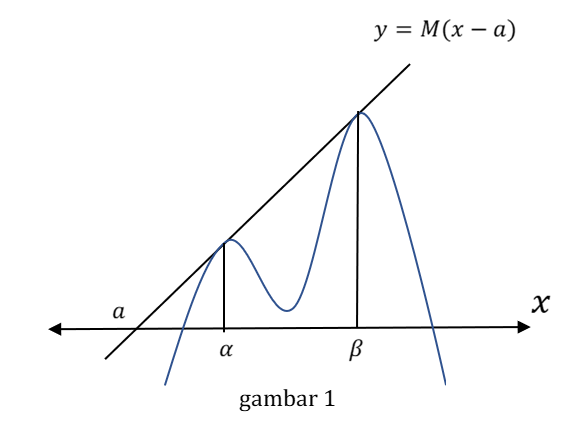
\includegraphics[width=0.27\textheight]{17(3)}
	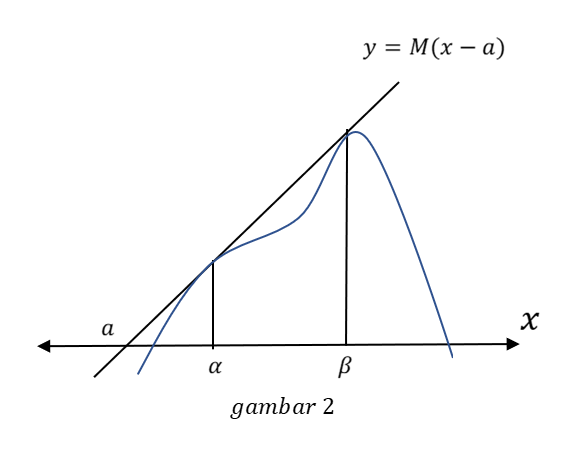
\includegraphics[width=0.27\textheight]{17(4)}\\
	Sekarang misalkan $r=\frac{\alpha+\beta}{2}$, karena $\beta-\alpha=6\sqrt{3}$, didapat $\alpha = r - 3\sqrt3$ dan $\beta = r +3\sqrt3$. Oleh karena itu persamaan (4) menjadi
	\begin{equation}
		h(x)=4(x-r)^3-108(x-r)
	\end{equation}
	Turunkan $h(x)$ terhadap $x$ didapat 
	\begin{equation}
		h'(x)=12(x-r+3)(x-r-3)
	\end{equation}
	Jika $h'(x)=0$ didapat $x=r-3$ atau $x=r+3$ yang mana berturut-turut merupakan absis dari titik maksimum lokal dan minimum lokal dari $h(x)$.
	Selanjutnya karena $y=h(x)$ memotong $y=M$ maksimal di dua titik dan $M>0$, berarti $M$ paling kecil adalah nilai maksimum lokal $h(x)$ atau $M \ge h(r-3)$ (seperti pada gambar 3). 
	\begin{figure}[h]
		\centering
		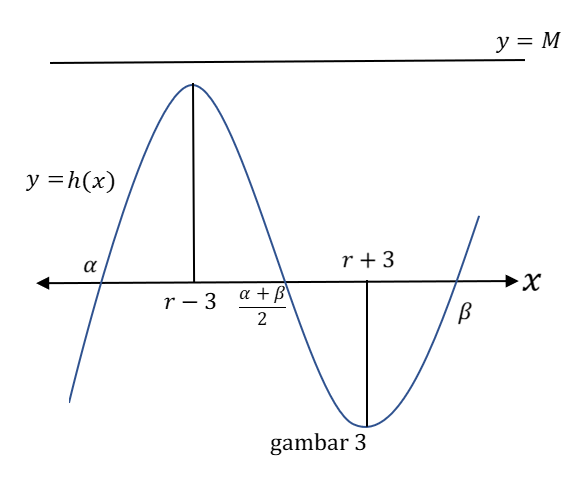
\includegraphics[width=0.3\textheight]{17(6)}
	\end{figure}
	\\
	Berarti dari persamaan (5) didapat
	$$M \ge h(r-3)=4(-3)^3-108(-3)=216$$
	Oleh karena itu didapat nilai minimum $M$ adalah 216. Kita selesai.
	
	

\end{document}